\chapter{Introdução}
Introdução

\section{\textit{Django}}
O \textit{Django} é um framework para desenvolvimento web. A linguagem de programação usada com esse framework é o Python.

O Python é uma linguagem de programação de alto nível, interpretada, imperativa, orientada a objetos, de tipagem dinâmica e forte. Foi lançada por Guido van Rossum em 1991.

A arquitetura utilizada no \textit{Django} basea-se no MTV (Model-Template-View), a qual diferencia-se um pouco do tradicional MVC (Model, View, Controller), arquitetura na qual separam-se as regras de negócios (Controller), os dados e métodos de acessos aos mesmos (Model) e as regras de apresentação (View).

No caso da arquitetura MTV, o framework \textit{Django} é o que faz as vezes de controlador da arquitetura MVC. Sendo assim, na arquitetura MTV, o Controller não é responsável pela lógica do negócio e sim pelo funcionamento do sistema. Além de models, views e templates, no \textit{Django} há também o URL dispatcher, middlewares e handlers e são estes que são encarados como Controller.

O URL dispatcher é o componente responsável em analisar os endereços requisitados pelo cliente e redirecionar essa requisição para a aplicação correta. Já o middleware é um conjunto de componentes que realizam pré e pós filtragens nas requisições, o que possibilita funcionalidade como internacionalização de uma aplicação e gerenciamento de sessões autenticadas.

No Model, são escritas as classes que designarão as tabelas no banco de dados. A manipulação dessas tabelas ocorre através do ORM (mapeamento objeto relacional) e, por isso, não é necessária a escrita de querys em SQL para a persistência dos dados.

A camada View consiste em uma função callback para uma respectiva URL descrevendo qual informação será fornecida. Pensando em separar as informações de suas apresentações foi criado a camada de Template, a qual descreve como as informações serão apresentadas para o usuário.

Com o uso do framework \textit{Django}, um projeto é um conjunto de aplicações. Uma aplicação é uma determinada funcionalidade que compõe um projeto. Por causa disso, há a idéia de aplicações plugáveis no \textit{Django} que é uma aplicação que pode ser usada em mais de um projeto com nenhuma ou quase nenhuma alteração de código. Isso quer dizer que a aplicação deve ter seus próprios modelos, suas próprias views, seus próprios templates e encapsular o máximo possível de código que não se enquadre em um desses elementos.

A Figura \ref{django-arq} ilustra a arquitetura do \textit{Django}:

\begin{figure}[h]
    \centering
    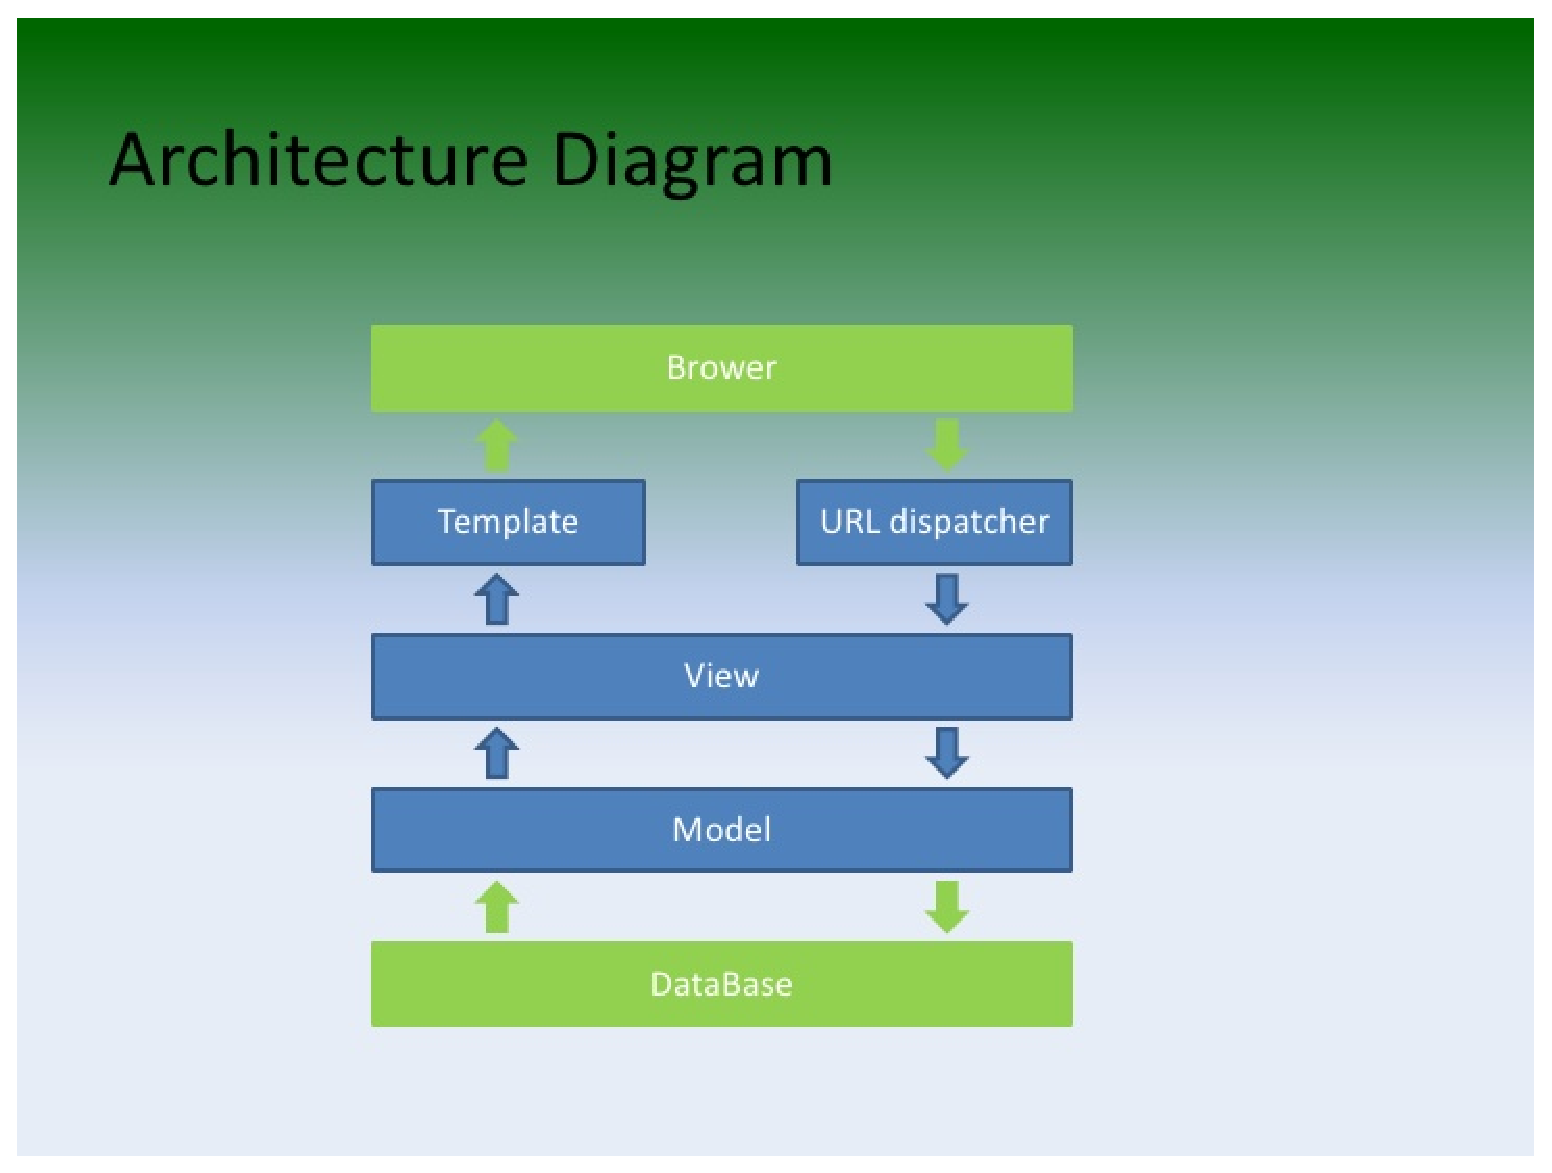
\includegraphics[keepaspectratio=true,scale=0.5]{figuras/django-arquitetura.eps}
    \caption{Arquitetura MTV \textit{Django}}
    \label{django-arq}
\end{figure}

\section{Pacotes Python Utilizados}
    \subsection{\textit{Coverage}}

    \subsection{\textit{GitLab CI}}

    \subsection{\textit{Matplotlib}}

    \subsection{\textit{Sphinx}}
    Ferramenta para criação inteligente e estilizada de documentação de códigos em \textit{python} e C/C++. Utiliza \textit{reStructuredText} como sua linguagem de marcação e converte toda a documentação
    para formato html, pdf, epub ou man.
